\documentclass[11pt]{article}
\renewcommand{\baselinestretch}{1.05}
\usepackage{amsmath,amsthm,verbatim,amssymb,amsfonts,amscd, graphicx}
\usepackage{graphics}
\topmargin0.0cm
\headheight0.0cm
\headsep0.0cm
\oddsidemargin0.0cm
\textheight23.0cm
\textwidth16.5cm
\footskip1.0cm
\theoremstyle{plain}

\usepackage{bm}

\usepackage{graphicx}


 \begin{document}

\title{Homework 1 Machine Learning}
\author{Marco Treglia}
\date{}
\maketitle

\section{K nearest neighbors}
K nearest neighbors is a simple algorithm that stores all available cases and classifies new cases based on a similarity measure (e.g., distance functions).
A case is classified by a majority vote of its neighbors, with the case being assigned to the class most common amongst its K nearest neighbors measured by a distance function.
\subsection{Metrics}
Distance fuction : 

$\bm{Euclidean  }$
$$d\; =\; \sqrt{\sum_{i\; =\; 1}^{k}{\left( x_{i}\; -\; y_{i} \right)^{2}}} $$


$\bm{Manhattan  }$
$$ d\; =\; \sum_{i\; =\; 1}^{k}{\left| x_{i}\; -\; y_{i} \right|} $$


$\bm{Minkowski  }$\footnote{With $p=1$ and $p=2$ rapprensent respectively Manhattan and  Euclidean distance }
$$d\; =\; \left( \sum_{i\; =\; 1}^{k}{\left( \left| x_{i}\; -\; y_{i} \right| \right)^{p}} \right)^{\frac{1}{p}} $$


\subsection{Weights}
One of the straight forward extension is not to give 1 vote to all the neighbors. A very common thing to do is weighted kNN where each point has a weight which is typically calculated using its distance. For eg under inverse distance weighting, each point has a weight equal to the inverse of its distance to the point to be classified. This means that neighboring points have a higher vote than the farther points. Weights : 
\\ \\
$\bm{Uniform  }$
\\
All points in each neighborhood are weighted equally.
\\ \\
$\bm{Distance  }$
\\
 Weight points by the inverse of their distance.
\\
\\
\\





\section{K nearest neighbors Visualizzation}


\subsection{Number of neighbors one to nine }

\begin{center}
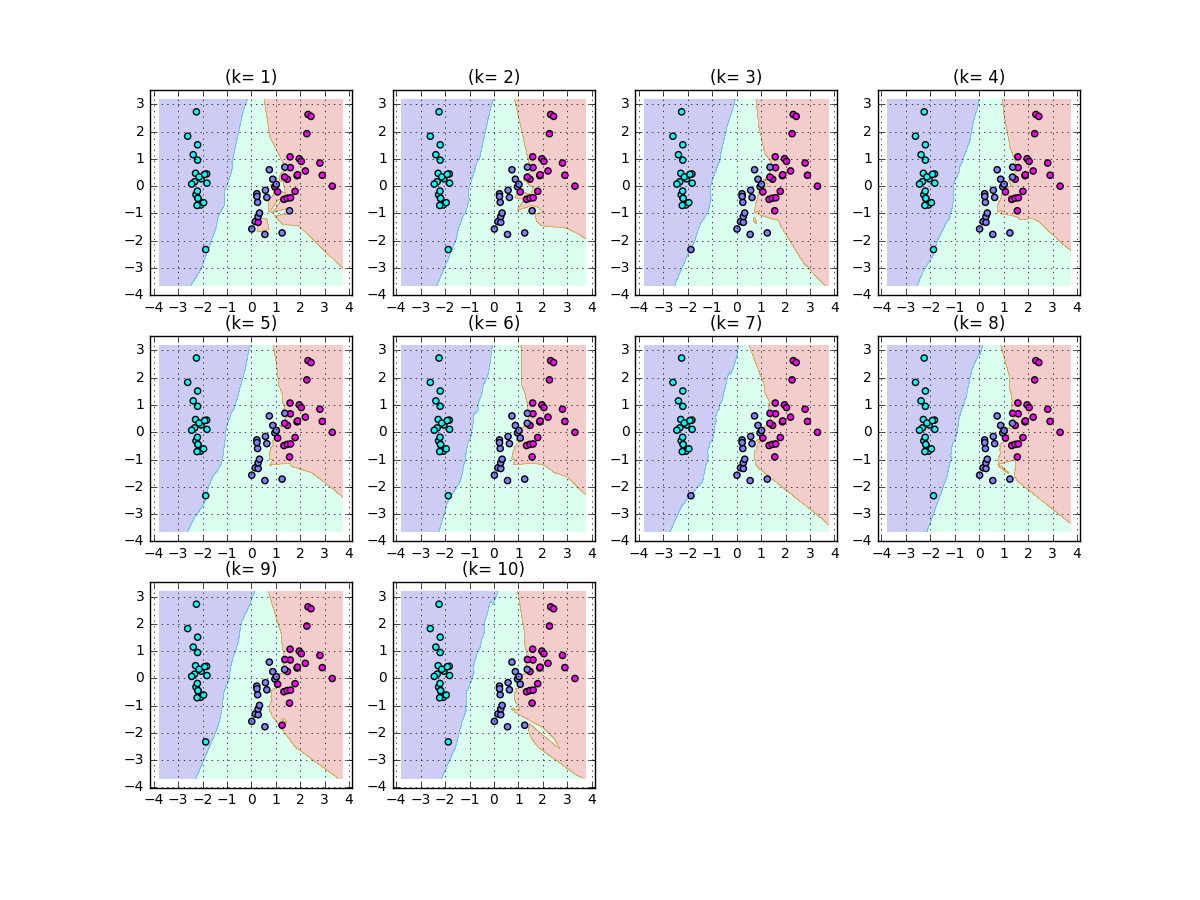
\includegraphics[scale=0.4]{0}
\end{center}

We can notice that the boundaries change for the result of considering respectly 1 to 10 neighbors for determinig at wich class the feature belong to. We can observe that if considering only one neighbor then we can be effected of overestimate the class with the noise of the data and considerign more neightbors the accuracy "might" increase but the computation cost also increases.


\begin{center}
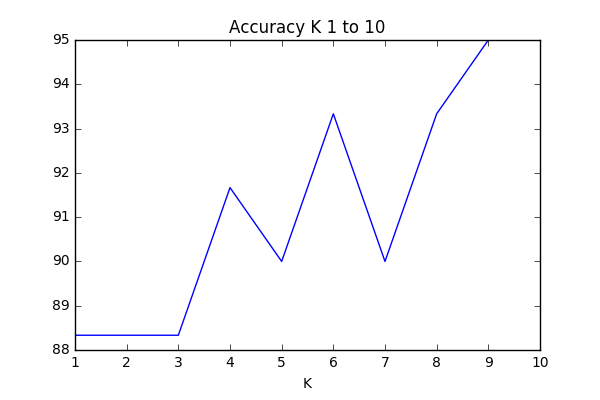
\includegraphics[scale=0.4]{1}
\end{center}
\begin{center}
Accurancy according the number of neighbors.
\end{center}

\subsection{Number of neighbors 3 with different weights fuction }

\begin{center}
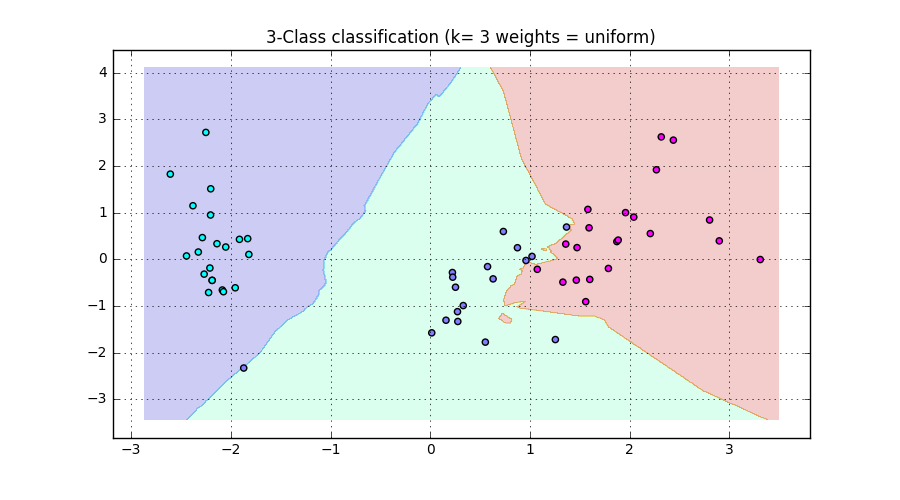
\includegraphics[scale=0.3]{2}
\end{center}

\begin{center}
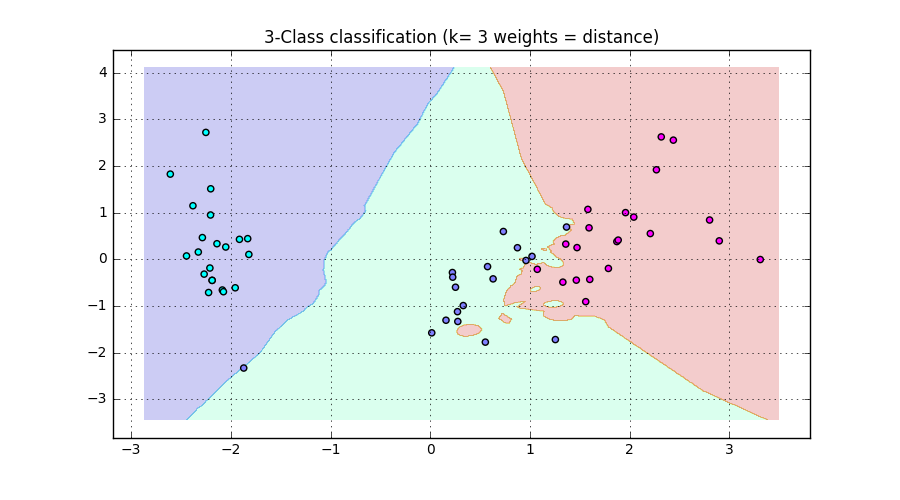
\includegraphics[scale=0.3]{3}
\end{center}

\begin{center}
 \begin{tabular}{||c c||} 
 \hline
 Weight &  Accuracy\\ [0.3ex] 
 \hline\hline
 Uniform &  88.33 \%  \\ 
 \hline
 Distance & 88.33 \%   \\
 \hline
\end{tabular}
\end{center}


\subsection{Gaussian function as weight function}

$$w\; =\; e^{-\alpha d^{2}} $$ 

\begin{center}
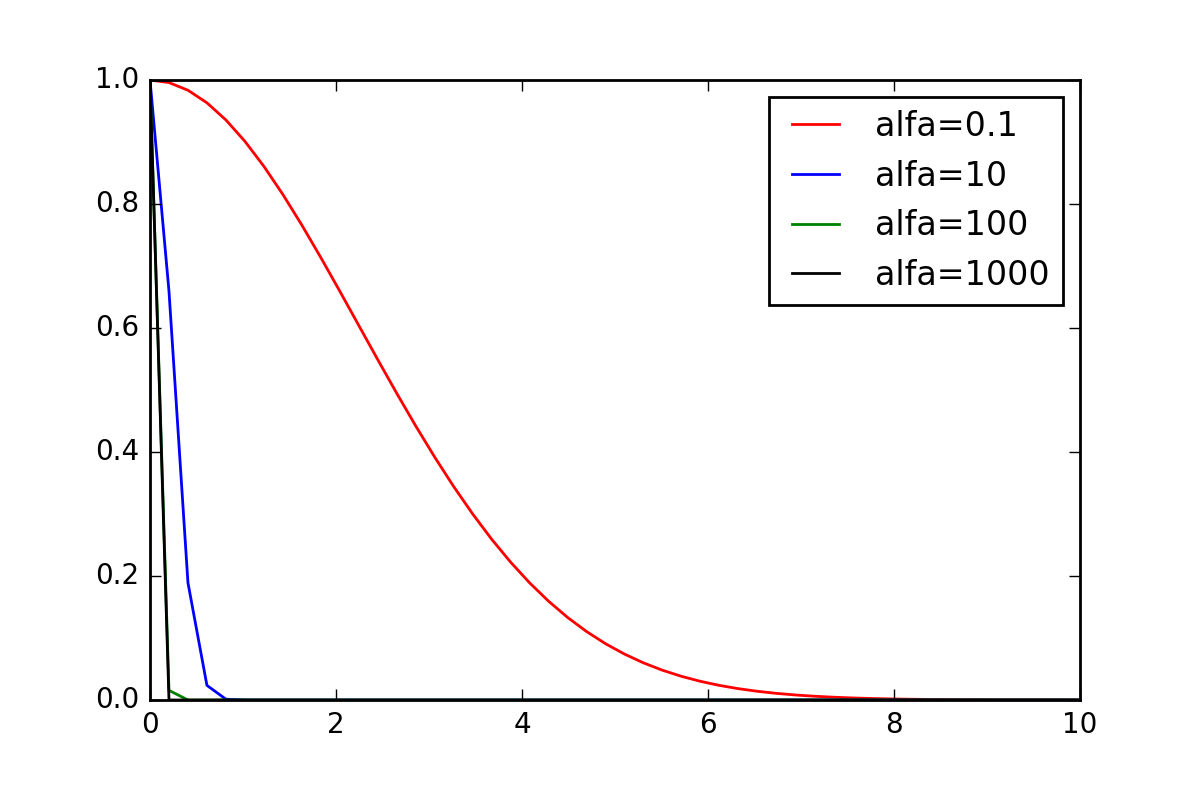
\includegraphics[scale=0.70]{gauss}
\end{center}
Distance is positive so the fuction is only decremental.


\begin{center}
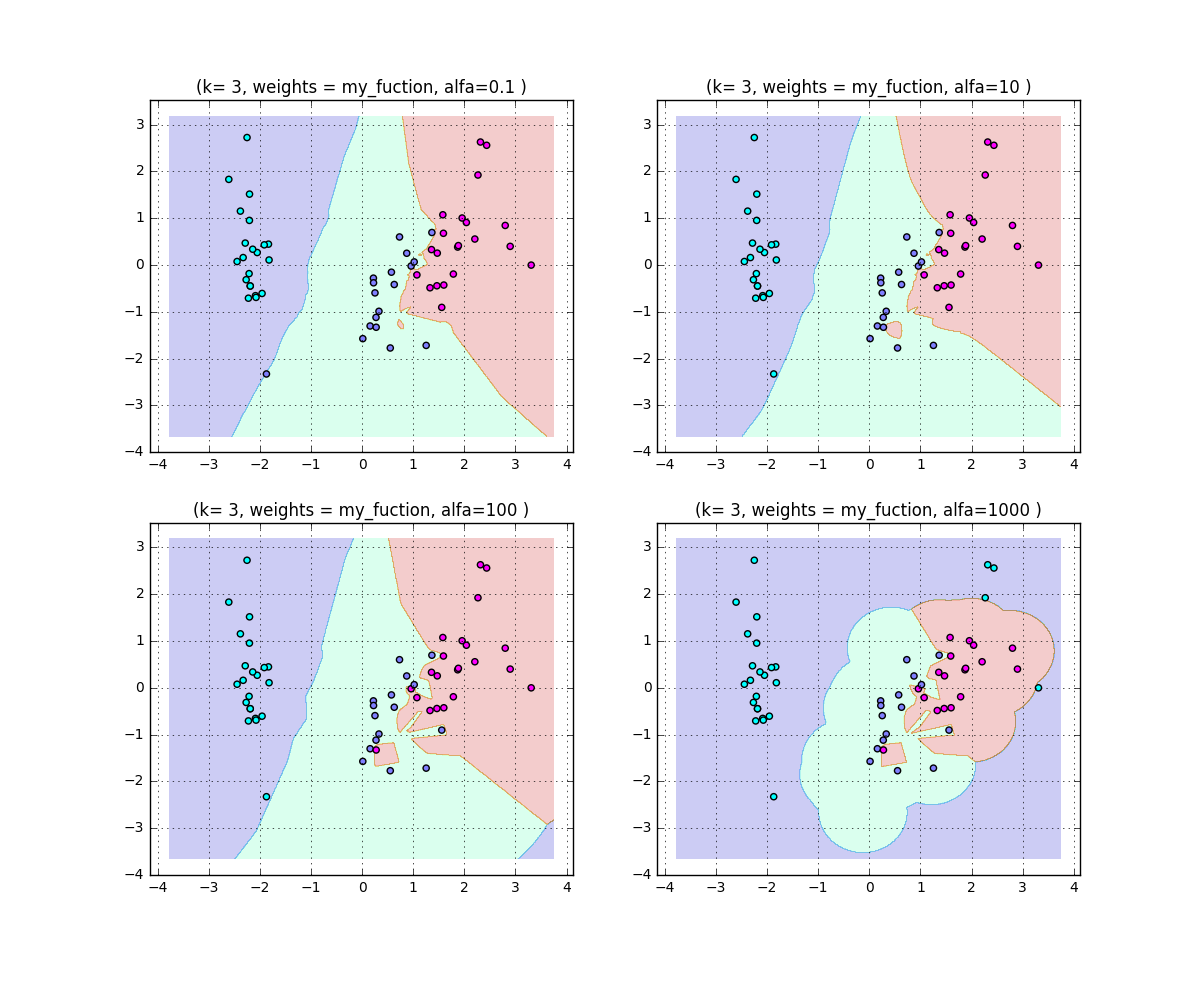
\includegraphics[scale=0.5]{4}
\end{center}

\begin{center}
Accuracy incrementing alfa . K = 3 
\end{center}

\begin{center}
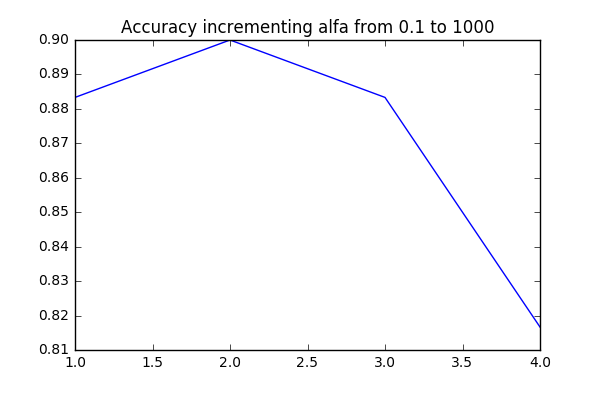
\includegraphics[scale=0.44]{5}
\end{center}

In this case we are using the gauss fuction as weight for estimante the k near neighbors , we can see that in the case of a big valuea of  $\alpha$ the fuction tend to zero faster then the case of the small one.
This means that when we are weighting the distance we can get some probability of commit an erroneous valutation. Infact, as shown at the end, the gauss fuction with a smaller value of $\alpha$ can predict with a nice accuracy. 
\\
\\
\\
\\
\subsection{Best solution finded with GridSearchCV}


\begin{center}
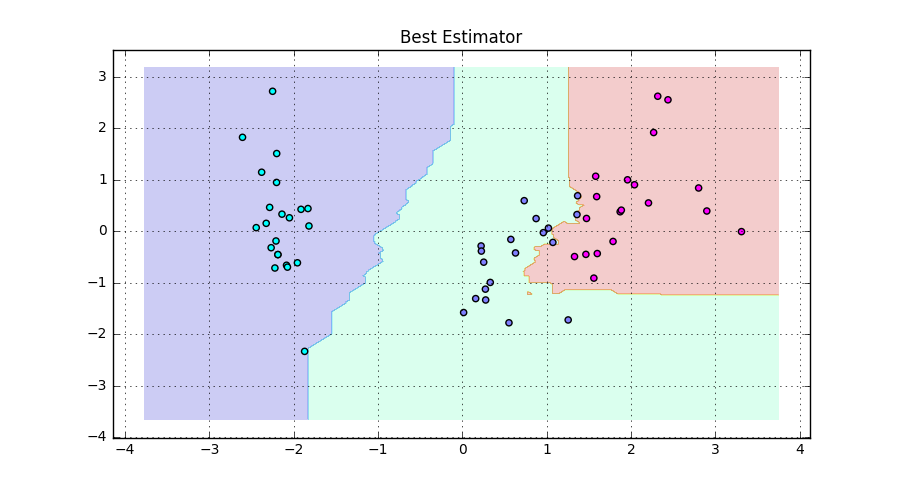
\includegraphics[scale=0.44]{6}
\end{center}

\begin{center}
Accuracy = 96.6 \%
\end{center}

After a grid search, the best parameter wich gives the higest accuracy are nine number of neightbors with a manhattan metric and the gaussian fuction as weight value.

\begin{center}
 \begin{tabular}{||c c c||} 
 \hline
  Number Neighbors & Weight &  Metric\\ [0.3ex] 
 \hline\hline
 9  &  Gaussian Func. &   Manhattan distance \\ 
 \hline

\end{tabular}
\end{center}

\end{document}